 \documentclass{homeworg}
\usepackage{amsmath}

\title{Travail 5 - Circuits RL}
\author{Wats Raphaël}

\begin{document}
\maketitle

\section{Schéma du circuit}
    \begin{center}
        \includegraphics[scale=0.38]{MainShematic.PNG}
    \end{center}
    
    Après observation, on observe que $R_5$ et $R_4$ sont en série car ils sont parcouru par le même courant. On peut donc simplifier le circuit de cette manière:
    \begin{center}
        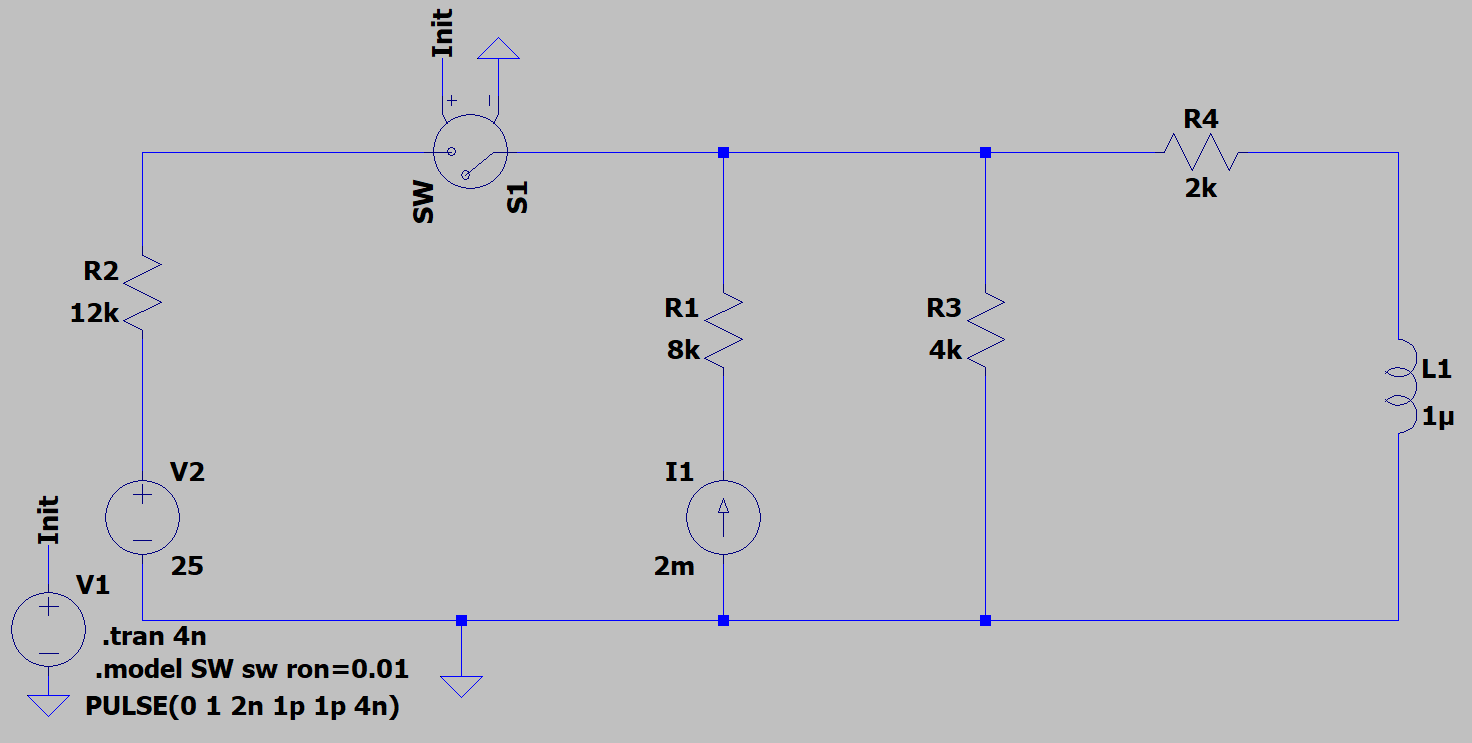
\includegraphics[scale=0.4]{Shematic.PNG}
    \end{center}

\newpage
\section{Le calcul de la condition initiale}
    \begin{center}
        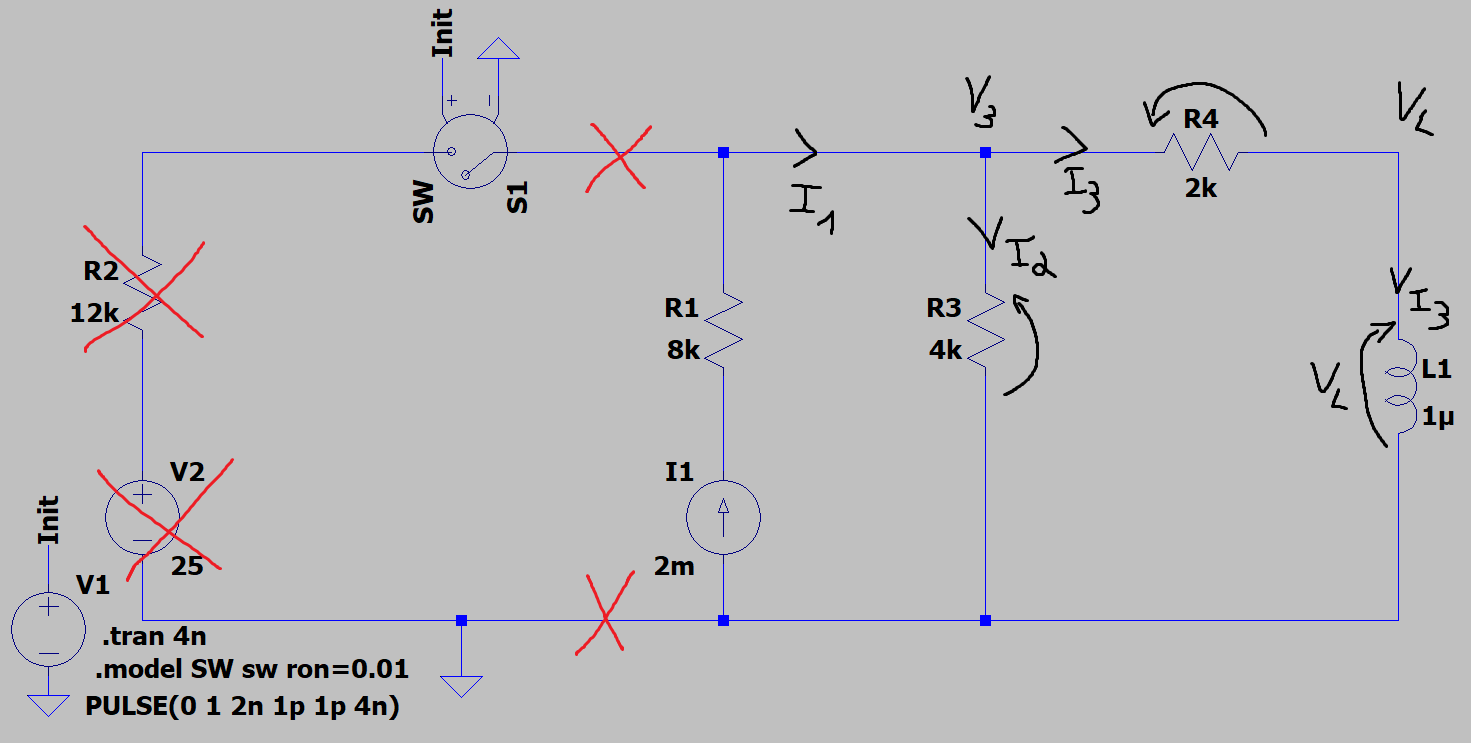
\includegraphics[scale=0.35]{Iinit.png}
    \end{center}
    Comme le circuit est ouvert, la résistance $R_2$ et la source tension $V_2$ ne sont pas actives, l'inductance elle est considérée comme un court-circuit donc $V_L = 0V$.
    \begin{align}
        V_L = 0\\
        I_1 = I_2 + I_3\\
        I_2 = V_3 / R_3\\
        I_3 = (V_3 - V_L) / R_4 = V_3 / R_4\\
        I_1 = V_3 / R_3 + V_3 / R_4\\
        V_3 = 2.67V\\
        I_3 = 2.67 / 2000 = 1.335mA
    \end{align}
    Le courant initial traversant l'inductance est donc $I_3 = 1.335mA$
\newpage
\section{Le calcul de la condition finale}
    \begin{center}
        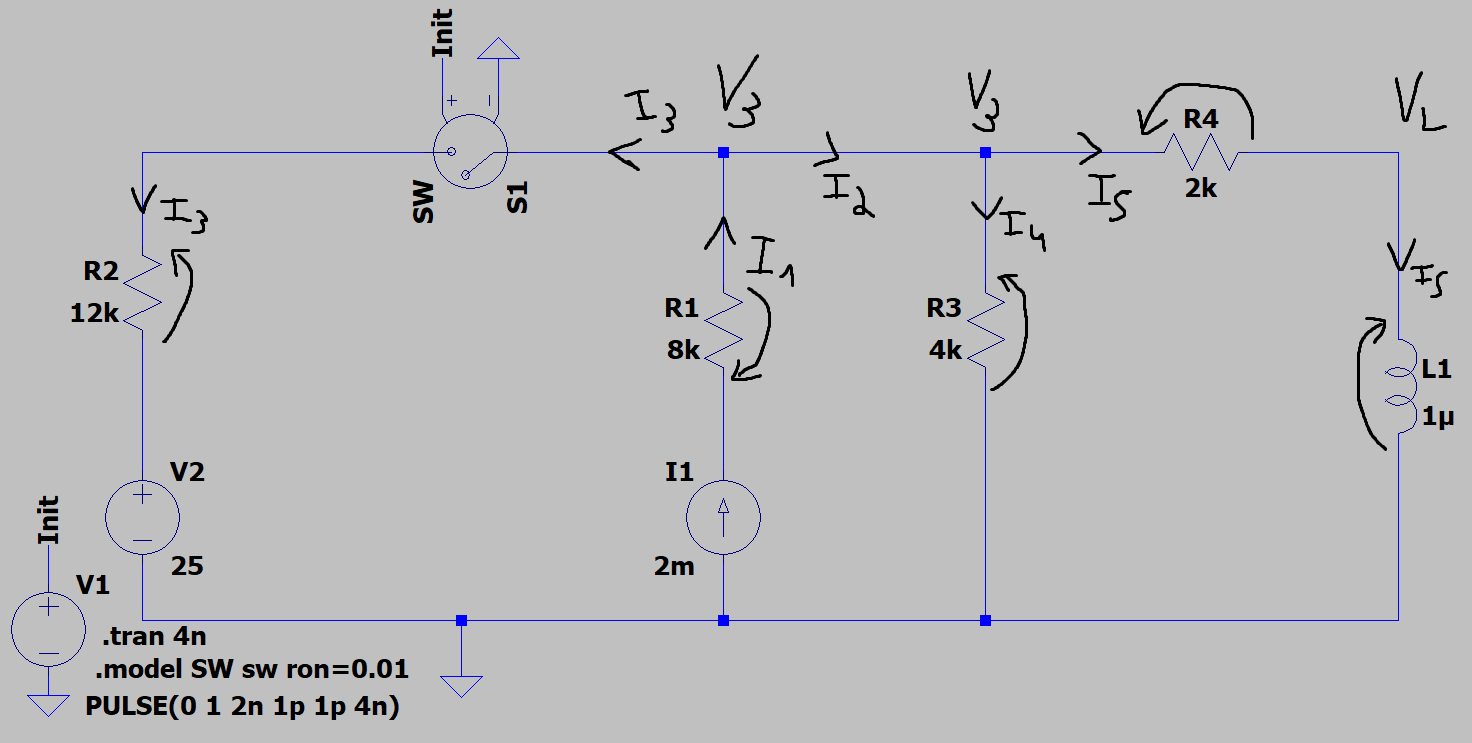
\includegraphics[scale=0.35]{Ifinal.png}
    \end{center}
    Comme le circuit est fermé, la résistance $R_2$ et la source tension $V_2$ sont à présent actives, l'inductance elle est considérée comme un court-circuit donc $V_L = 0V$.
    \begin{align}
        V_L = 0\\
        I_1 = I_2 + I_3\\
        I_2 = I_4 + I_5\\
        I_3 = (V_3 - V_2) / R_2\\
        I_4 = V_3 / R_3\\
        I_5 = (V_3 - V_L) / R_4 = V_3 / R_4\\
        I_2 = V_3 / R_3 + V_3 / R_4\\
        I_1 = V_3 / R_3 + V_3 / R_4 + (V_3 - V_2) / R_2\\
        V_3 = 4.9V\\
        I_5 = 4.9V / 2000 = 2.45mA
    \end{align}

\section{Le calcul de la constante de temps}
$\tau = L / R_{eq}$, où $R_{eq}$ est la résistance équivalente vu par l'inductance $R_{eq} = (R_2 // R_3) + R_4 = 5k\Omega$ et L est la valeur de l'inductance. $\tau = 1\mu / 5k\Omega = 0.2n$ secondes.

\section{Le calcul du courant dans l'inductance}
L’équation diférentielle du premier ordre pour calculer le courant dans l'inductance est:
\begin{align}
     I_L(t) = A + B e^{-t / \tau}
\end{align}

On a alors, $I_L(t=0) = 1.335mA$ à la condition initial et $I_L(t=\infty)= 2.45mA$ à la condition finale
\begin{align}
    I_L(0) = A + B e^{0/ \tau} = 1.335mA\\
    I_L(\infty) = A + B e^{-\infty/ \tau} = 2.45mA
\end{align}

Grâce à la relation [5.2] on peut exprimer B en terme de A:
\begin{align}
    I_L(0) = A + B e^{0/ \tau} = 1.335mA\\
    I_L(0) = A + B e^{0} = 1.335mA\\
    I_L(0) = A + B * 1 = 1.335mA\\
    I_L(0) = A + B = 1.335mA\\
    B = 1.335mA - A
\end{align}

On obtient la valeur de A Grâce à la relation [5.3]
\begin{align}
    I_L(\infty) = A + B e^{-\infty/ \tau} = 2.45mA\\
    I_L(\infty) = A + B * (1/e^{\infty/ \tau}) = 2.45mA\\
    I_L(\infty) = A + B * 0 = 2.45mA\\
    I_L(\infty) = A = 2.45mA
\end{align}

Grâce à la relation [5.8] on obtient $A = 2.45mA$ et $B = -1.115mA$ on obtient alors grâce la relation [5.1] l'expression du courant dans l'inductance en fonction du temps.
\begin{align}
    I_L(t) = (2.45 - 1.115e^{-t / \tau}) * 10^{-3}
\end{align}

On peut à présent vérifier nos résultats grâce à la simulation !
Pour $t=0.1n$ secondes (on sera alors à 2.1n secondes sur notre simulation) on aura:
\begin{align}
    -t / \tau = -0.1 * 10^{-9} / 0.2 * 10^{-9} = -1/2 = -0.5\\
    I_L(0.1 * 10^{-9}) = (2.45 - 1.115e^{-0.5}) * 10^{-3} = 1.77mA
\end{align}


\begin{center}
    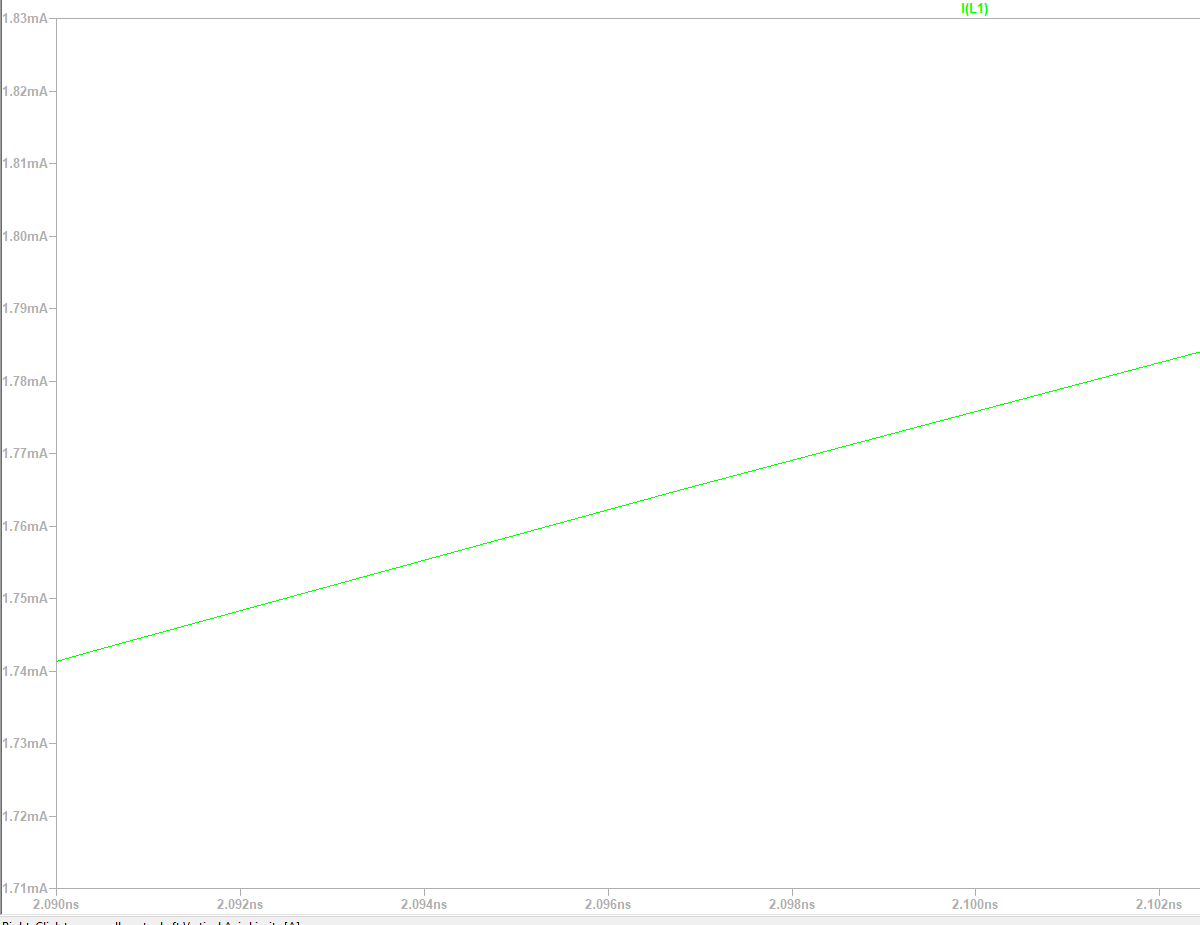
\includegraphics[scale=0.35]{CurentPoint.PNG}
\end{center}

\newpage
\section{Le calcul de la tension aux bornes de l'inductance}
    La tension aux bornes de l'inductance est donné par la relation:
    \begin{align}
        V_L(t) = L * I_L(t)'\\
        V_L(t) = 10^{-6} * 1.115/\tau * e^{-t/\tau} * 10^{-3}\\
        V_L(T) = 1.115/\tau * e^{-t/\tau} * 10^{-9} 
    \end{align}
    Où L est la valeur de l'inductance et $I_L(t)'$ est la dérivée de la fonction qui donne le courant de l'inductance en fonction du temps.
    
    Pour $t=0.1n$ secondes (on sera alors à 2.1n secondes sur notre simulation) on aura:
    \begin{align}
        -t / \tau = -0.1 * 10^{-9} / 0.2 * 10^{-9} = -1/2 = -0.5\\
        V_L(0.1 * 10^{-9}) = 1.115/0.2 * e^{-0.5}\\
        V_L(0.1n) = 3.38V
    \end{align}
    \begin{center}
        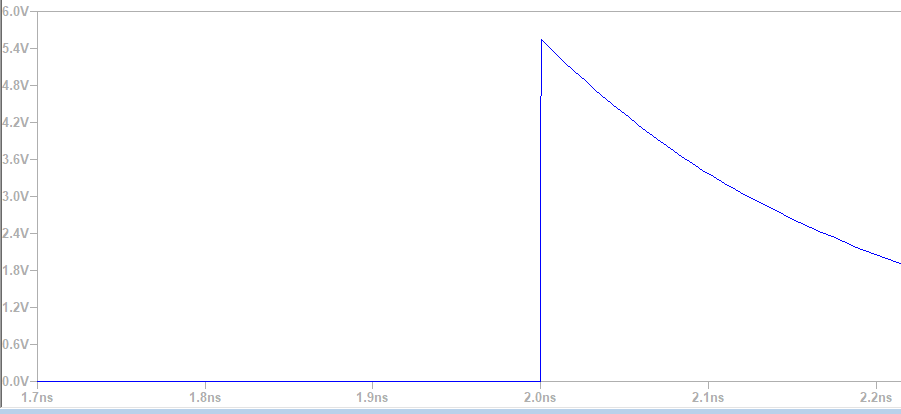
\includegraphics[scale=0.6]{VoltagePoint.PNG}
    \end{center}
\newpage
\section{La simulation du circuit}
\begin{center}
        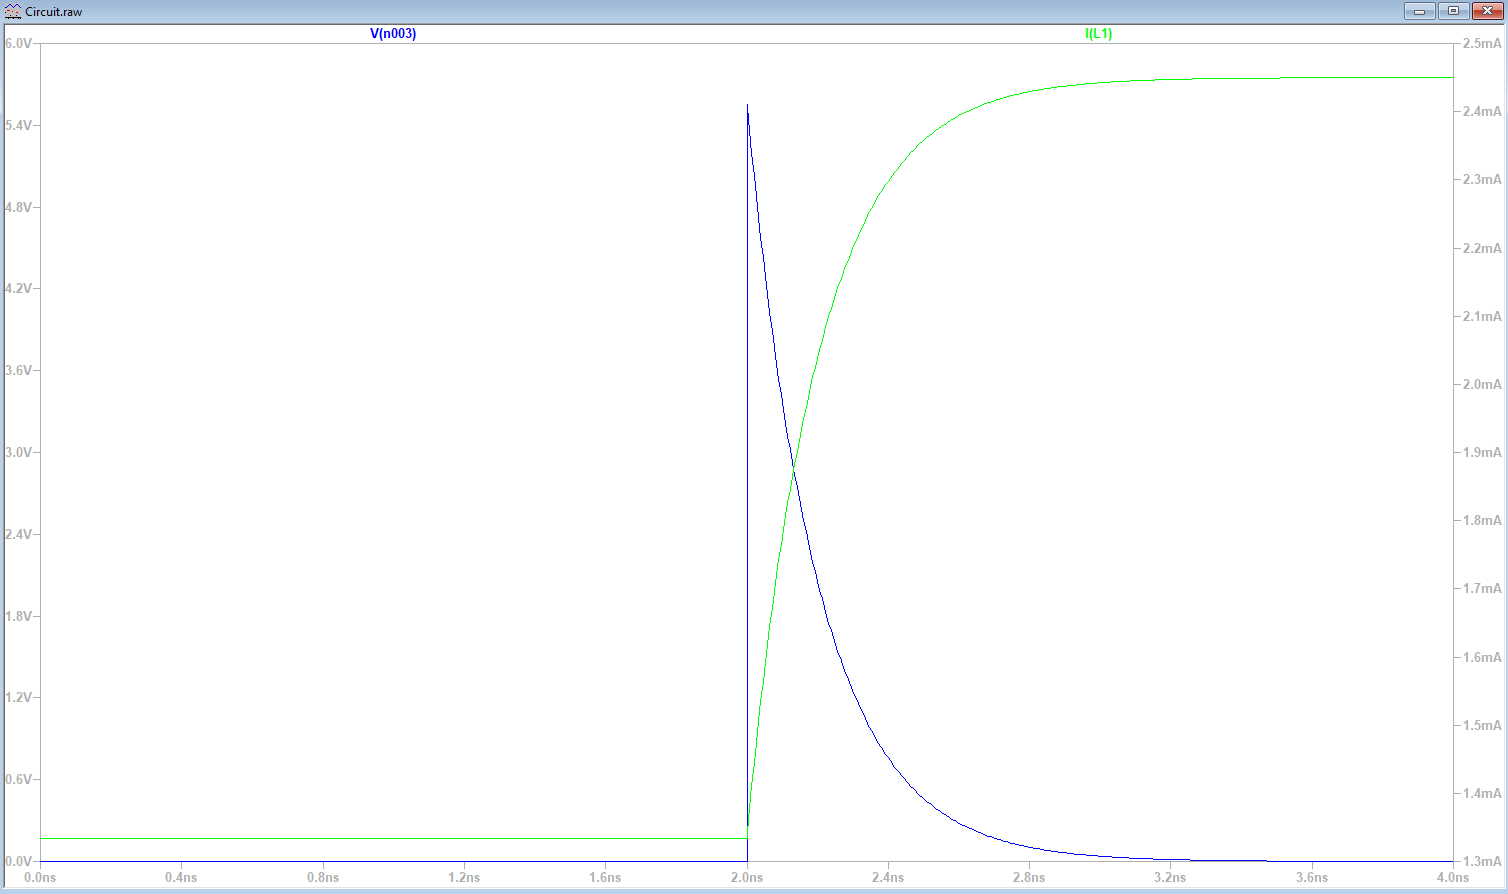
\includegraphics[scale=0.3]{Simu.PNG}
\end{center}
Ici on observe bien l'exemple d'un circuit transitoire où la tension et le courant évolue en fonction du temps

\section{Conclusion}
    Les résultats obtenu sont en adéquation avec ceux obtenu lors de la simulation LTspice XVII.
    \begin{itemize}
        \item On observe que la tension aux bornes de l'inductance ainsi que le courant évolue en fonction du temps d'où le nom de régime transitoire.
    \end{itemize}
\end{document}
